\documentclass{article}\usepackage{graphicx, color}
%% maxwidth is the original width if it is less than linewidth
%% otherwise use linewidth (to make sure the graphics do not exceed the margin)
\makeatletter
\def\maxwidth{ %
  \ifdim\Gin@nat@width>\linewidth
    \linewidth
  \else
    \Gin@nat@width
  \fi
}
\makeatother

\definecolor{fgcolor}{rgb}{0.2, 0.2, 0.2}
\newcommand{\hlnumber}[1]{\textcolor[rgb]{0,0,0}{#1}}%
\newcommand{\hlfunctioncall}[1]{\textcolor[rgb]{0.501960784313725,0,0.329411764705882}{\textbf{#1}}}%
\newcommand{\hlstring}[1]{\textcolor[rgb]{0.6,0.6,1}{#1}}%
\newcommand{\hlkeyword}[1]{\textcolor[rgb]{0,0,0}{\textbf{#1}}}%
\newcommand{\hlargument}[1]{\textcolor[rgb]{0.690196078431373,0.250980392156863,0.0196078431372549}{#1}}%
\newcommand{\hlcomment}[1]{\textcolor[rgb]{0.180392156862745,0.6,0.341176470588235}{#1}}%
\newcommand{\hlroxygencomment}[1]{\textcolor[rgb]{0.43921568627451,0.47843137254902,0.701960784313725}{#1}}%
\newcommand{\hlformalargs}[1]{\textcolor[rgb]{0.690196078431373,0.250980392156863,0.0196078431372549}{#1}}%
\newcommand{\hleqformalargs}[1]{\textcolor[rgb]{0.690196078431373,0.250980392156863,0.0196078431372549}{#1}}%
\newcommand{\hlassignement}[1]{\textcolor[rgb]{0,0,0}{\textbf{#1}}}%
\newcommand{\hlpackage}[1]{\textcolor[rgb]{0.588235294117647,0.709803921568627,0.145098039215686}{#1}}%
\newcommand{\hlslot}[1]{\textit{#1}}%
\newcommand{\hlsymbol}[1]{\textcolor[rgb]{0,0,0}{#1}}%
\newcommand{\hlprompt}[1]{\textcolor[rgb]{0.2,0.2,0.2}{#1}}%

\usepackage{framed}
\makeatletter
\newenvironment{kframe}{%
 \def\at@end@of@kframe{}%
 \ifinner\ifhmode%
  \def\at@end@of@kframe{\end{minipage}}%
  \begin{minipage}{\columnwidth}%
 \fi\fi%
 \def\FrameCommand##1{\hskip\@totalleftmargin \hskip-\fboxsep
 \colorbox{shadecolor}{##1}\hskip-\fboxsep
     % There is no \\@totalrightmargin, so:
     \hskip-\linewidth \hskip-\@totalleftmargin \hskip\columnwidth}%
 \MakeFramed {\advance\hsize-\width
   \@totalleftmargin\z@ \linewidth\hsize
   \@setminipage}}%
 {\par\unskip\endMakeFramed%
 \at@end@of@kframe}
\makeatother

\definecolor{shadecolor}{rgb}{.97, .97, .97}
\definecolor{messagecolor}{rgb}{0, 0, 0}
\definecolor{warningcolor}{rgb}{1, 0, 1}
\definecolor{errorcolor}{rgb}{1, 0, 0}
\newenvironment{knitrout}{}{} % an empty environment to be redefined in TeX

\usepackage{alltt}
\usepackage{geometry}
\geometry{left=1.25in,right=1in,top=1.25in,bottom=1.25in}
\setlength\parindent{0pt}
\IfFileExists{upquote.sty}{\usepackage{upquote}}{}
\begin{document}
\section*{Question 5}
Since we have a very small number of variables we will do 'classical' model selection by starting with the saturated model and seeing if we can remove the interaction term.




\begin{knitrout}
\definecolor{shadecolor}{rgb}{0.969, 0.969, 0.969}\color{fgcolor}\begin{kframe}
\begin{alltt}
m2 = \hlfunctioncall{lm}(LATE ~ BILL * TYPE)
\hlfunctioncall{summary}(m2)$coef
\end{alltt}
\begin{verbatim}
##                      Estimate Std. Error t value  Pr(>|t|)
## (Intercept)          101.7582   1.198504   84.90 3.475e-89
## BILL                  -0.1910   0.006285  -30.38 9.386e-50
## TYPERESIDENTIAL      -99.5486   1.694940  -58.73 9.905e-75
## BILL:TYPERESIDENTIAL   0.3566   0.008888   40.13 4.370e-60
\end{verbatim}
\end{kframe}
\end{knitrout}


We see that we need to include all covariates in our model by the small values of the wald tests. Next we will do model checking to make sure we have a good fit. First we will check for patterns in our residuals.

\begin{knitrout}
\definecolor{shadecolor}{rgb}{0.969, 0.969, 0.969}\color{fgcolor}\begin{kframe}
\begin{alltt}

\hlfunctioncall{plot}(BILL, m2$resid)
\hlfunctioncall{ggplot}(data, \hlfunctioncall{aes}(x = TYPE, y = m2$resid)) + \hlfunctioncall{geom_boxplot}()
\end{alltt}
\end{kframe}
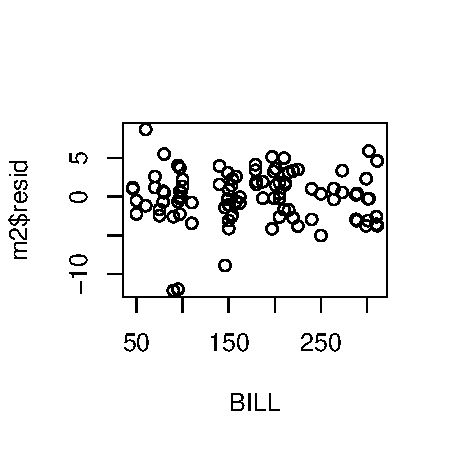
\includegraphics[width=\maxwidth]{figure/unnamed-chunk-31} 
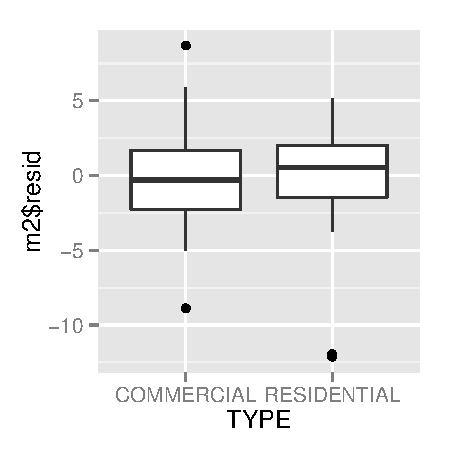
\includegraphics[width=\maxwidth]{figure/unnamed-chunk-32} 

\end{knitrout}



With no obvious patterns in the resudials, we will now check for outliers

\begin{knitrout}
\definecolor{shadecolor}{rgb}{0.969, 0.969, 0.969}\color{fgcolor}\begin{kframe}
\begin{alltt}
\hlfunctioncall{plot}(\hlfunctioncall{fitted}(m2), \hlfunctioncall{studres}(m2))
\hlfunctioncall{qqnorm}(\hlfunctioncall{studres}(m2))
\hlfunctioncall{qqline}(\hlfunctioncall{studres}(m2))
\end{alltt}
\end{kframe}
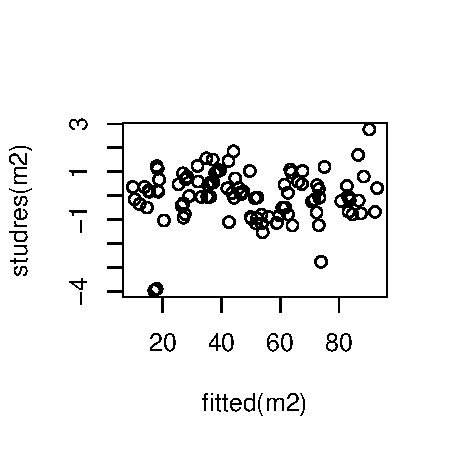
\includegraphics[width=\maxwidth]{figure/unnamed-chunk-41} 
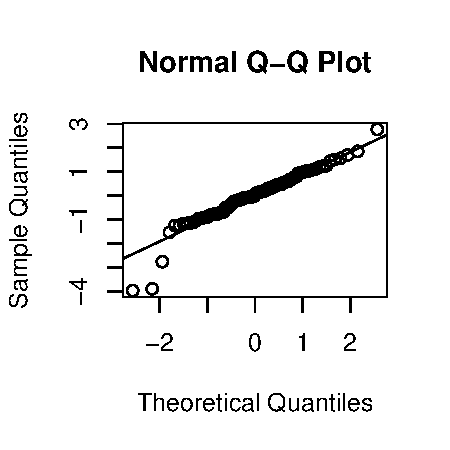
\includegraphics[width=\maxwidth]{figure/unnamed-chunk-42} 

\end{knitrout}

Although a couple of points may arguably be outliers, we will keep them in the model as they are not too bad and the outliers are unlikely to change the estimates of the model. Next we will check for poitns of influence


\begin{knitrout}
\definecolor{shadecolor}{rgb}{0.969, 0.969, 0.969}\color{fgcolor}\begin{kframe}
\begin{alltt}
\hlfunctioncall{sort}(\hlfunctioncall{lm.influence}(m2)$hat)[1:10]
\end{alltt}
\begin{verbatim}
##      46      54      90      23      33      87      28      86      20 
## 0.02091 0.02091 0.02095 0.02095 0.02136 0.02136 0.02140 0.02140 0.02175 
##      59 
## 0.02175
\end{verbatim}
\end{kframe}
\end{knitrout}

We see that there are no influencial points. Now that we are satisfied with our model we can interpret it. Recall the parameters
\begin{knitrout}
\definecolor{shadecolor}{rgb}{0.969, 0.969, 0.969}\color{fgcolor}\begin{kframe}
\begin{alltt}
\hlfunctioncall{coef}(m2)
\end{alltt}
\begin{verbatim}
##          (Intercept)                 BILL      TYPERESIDENTIAL 
##             101.7582              -0.1910             -99.5486 
## BILL:TYPERESIDENTIAL 
##               0.3566
\end{verbatim}
\end{kframe}
\end{knitrout}

Which we can interpret as follows.
For a commercial building with a small bill, we will have to wait about 100 days. For a residental building with a small bill we will have to wait about 0 days. As the bill increases by one, we wil expect to wait .2 less days for a commercial building, and .15 more days for a residental building. We can plot these regression lines as follows.

\begin{knitrout}
\definecolor{shadecolor}{rgb}{0.969, 0.969, 0.969}\color{fgcolor}\begin{kframe}
\begin{alltt}
\hlfunctioncall{ggplot}(data, \hlfunctioncall{aes}(x = BILL, y = LATE, shape = TYPE)) + \hlfunctioncall{geom_point}() + \hlfunctioncall{stat_smooth}(method = lm)
\end{alltt}
\end{kframe}
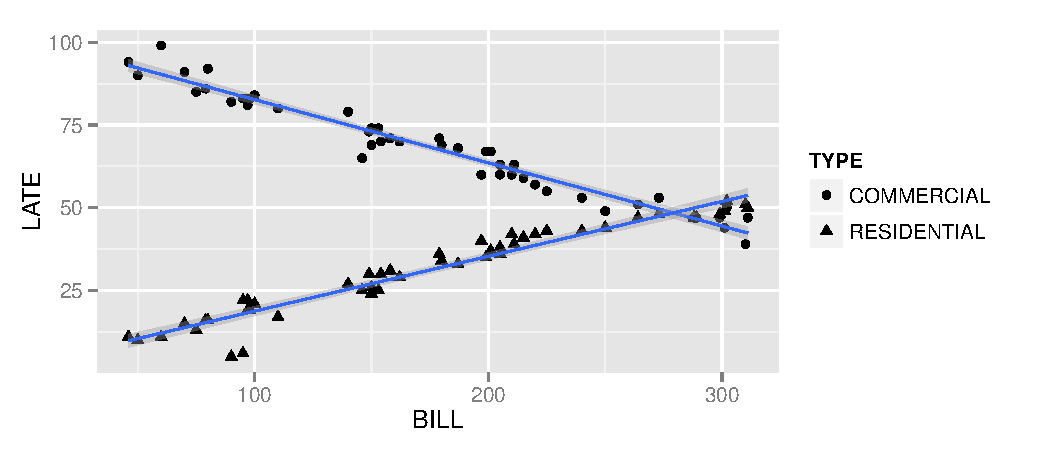
\includegraphics[width=\maxwidth]{figure/unnamed-chunk-7} 

\end{knitrout}


Using this plot we can say that the marketing department should make different claims for commercial and residential clients. It seems they can indeed they can collect most of their residential claims in 60 days, however they are unlikely to collect their commercial claims in 60 days. In order to balance simplicity and accuracy I would make the following four claims.

\begin{itemize}
\item Residential claims under \$150 can be collected in 30 days
\item Residential claims over \$150 can be collected in 60 days
\item Commercial claims over \$150 can be collected in 75 days
\item Commercial claims under \$150 can be collected in 100 days
\end{itemize}

\end{document}
